\chapter{排版格式}\label{chap:format}

\section{引言}
依据中华人民共和国《科学技术报告、学位论文和学术论文的编写格式》和东北大学学位论文格式改编,专为我校申请硕士、博士学位人员撰写打印论文时使用。本格式自发布日起实行。
\section{学位论文主要部分}
学位论文主要部分由前头部分、主体部分和结尾部分组成。
\subsection{前头部分}
\begin{itemize}
    \item 封面
    \item 扉页——题名页(中、英两种)
    \item 声明(独创性声明)
    \item 摘要(中、英两种文字)
    \item 目录
    \item 插图和附表清单(只限必要时)
    \item 缩略字、缩写词、符号、单位表(只限必要时)
    \item 名词术语注释表(只限必要时)
\end{itemize}

\subsection{主体部分}
\begin{itemize}
    \item 绪论(前言、引言、绪言)
    \item 正文
    \item 讨论、结论和建议
\end{itemize}
\subsection{结尾部分(只限必要时采用)}
\begin{itemize}
    \item 参考文献
    \item 致谢
    \item 攻读博士学位期间取得的学术成果
    \item 作者从事科学研究和学习经历的简历
    \item 可供参考的文献题录(只限必要时采用)
    \item 索引(只限必要时采用)
\end{itemize}

\section{版式}
纸张大小:纸的尺寸为标准A4复印纸(210mm×297mm)。

版芯(打印尺寸):160mm×247mm(不包括页眉行、页码行)。

正文字体字号:小4号宋体,全文统一。

每页30~35行,每行35~38字。

装订:双面打印印刷,沿长边装订。

页码:页码用阿拉伯数字连续编页,字号与正文字体相同,页底居中,数字两侧用圆点或一字横线修饰,如·3·或-3-。

页眉:自摘要页起加页眉,眉体可用单线或双线(二等线、文武线),页眉说明5号楷体,左端“东北大学硕士、博士学位论文”,右端“章号章题”。

封面:东北大学研究生(博士或硕士)学位论文标准封面(双A4)。

\section{体例}

\subsection{标题}

论文正文按章、条、款、项分级,在不同级的章、条、款、项阿拉伯数字编号之间用点“.”(半角实心下圆点)相隔,最末级编号之后不加点。排版格式见表4.1。

此分级编号法只分至第四级。再分可用(1)、(2)……;(a)、(b)……等。

\begin{table}[htpb]
    \begin{center}
        \bicaption{标题排版格式}{Typesetting format of the heading}
        \begin{tabular}{|l | l | l | l |}
            \hline
            标题       & 字号字体   & 格式        & 举例           \\
            \hline
            第一级(章) & 二号黑体   & 居中,占3行 & 第1章 XXX      \\
            \hline
            第二级(条) & 三号黑体   & 居左,占2行 & 1.1 XXXXXX     \\
            \hline
            第三级(款) & 四号黑体   & 居左,占2行 & 1.1.1 XXXXXX   \\
            \hline
            第四级(项) & 小四号黑体 & 居左,占1行 & 1.1.1.1 XXXXXX \\
            \hline
        \end{tabular}
    \end{center}
\end{table}

摘要、目录、参考文献、致谢、攻读博士学位期间取得的学术成果、个人简历等标题作为第一级标题排版。

\subsection{正文}
汉字字体字号:正文字体小4号宋体。

外文、数字字号与同行汉字字号相同,字体用WORD系统中的Time New Roman体或相近字体。

\subsubsection{插图}
插图包括图解、示意图、构造图、曲线图、框图、流程图、布置图、地图、照片、图版等。插图注明项有图号、图题、图例。图号编码用章序号。如“图2.1“表示第2章第1图。图号与图题文字间置一字空格,置于图的正下方,图题用5号字,字体可用宋体,须全文统一。图中标注符号文字字号不大于图题的字号。

论文中图片的插入通常分为单图和多图,下面分别加以介绍:

单图插入:假设插入名为\verb|tc_q_criteria|(后缀可以为.jpg、.png、.pdf,下同)的图片,其效果如图\ref{fig:tc_q_criteria}。
\begin{figure}[!htbp]
    \centering
    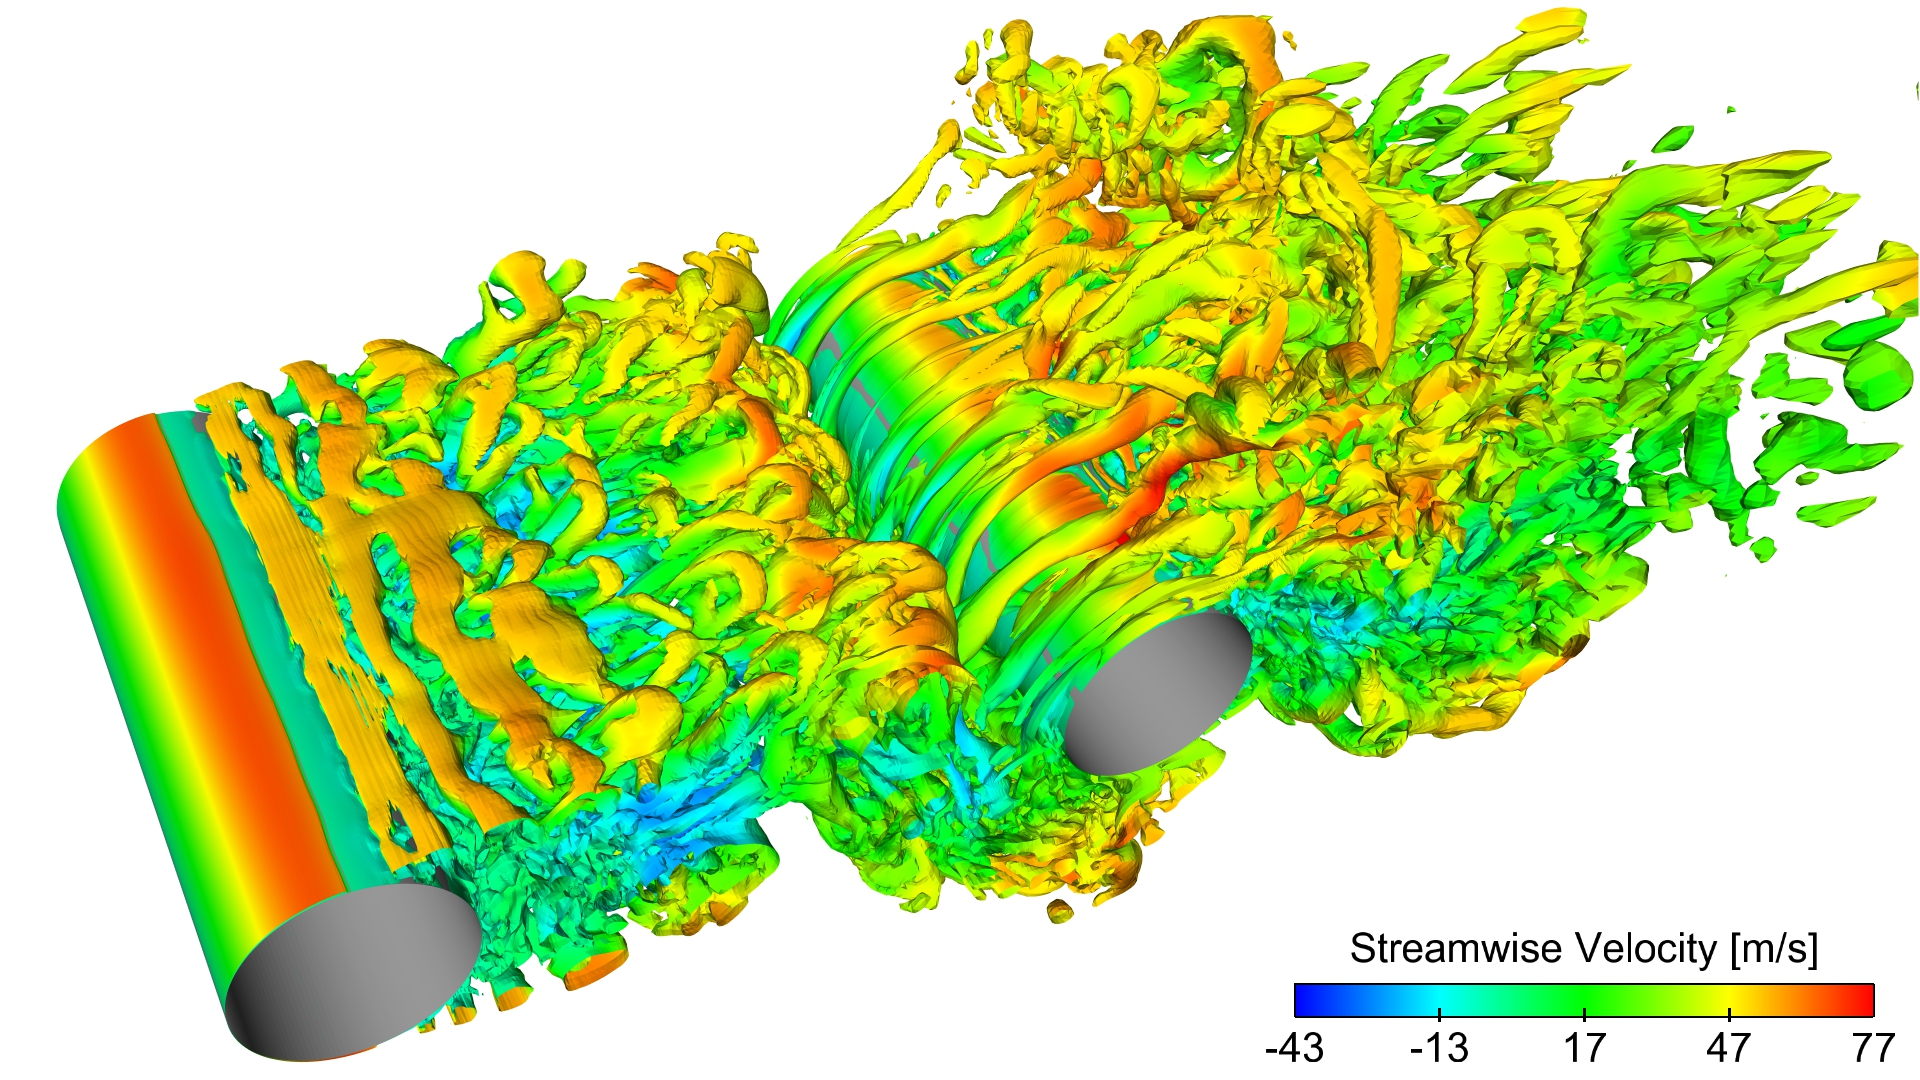
\includegraphics[width=0.40\textwidth]{tc_q_criteria}
    \bicaption{Q判据等值面图,同时测试一下一个很长的标题,比如这真的是一个很长很长很长很长很长很长很长很长的标题。}{Isocontour of Q criteria, at the same time, this is to test a long title, for instance, this is a really very long very long very long very long very long title.}
    \label{fig:tc_q_criteria}
\end{figure}

如果插图的空白区域过大,以图片\verb|shock_cyn|为例,自动裁剪如图\ref{fig:shock_cyn}。
\begin{figure}[!htbp]
    \centering
    %trim option's parameter order: left bottom right top
    % 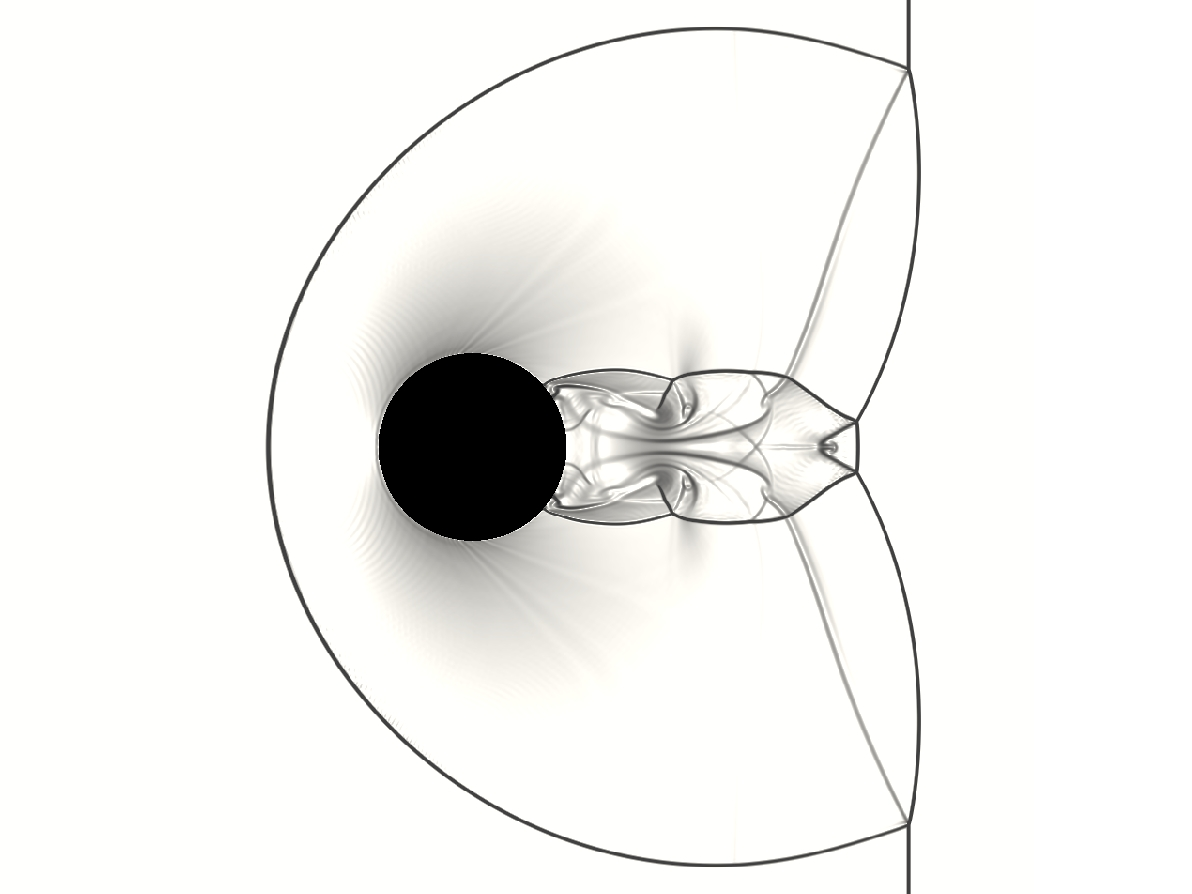
\includegraphics[trim = 30mm 0mm 30mm 0mm, clip, width=0.40\textwidth]{shock_cyn}
    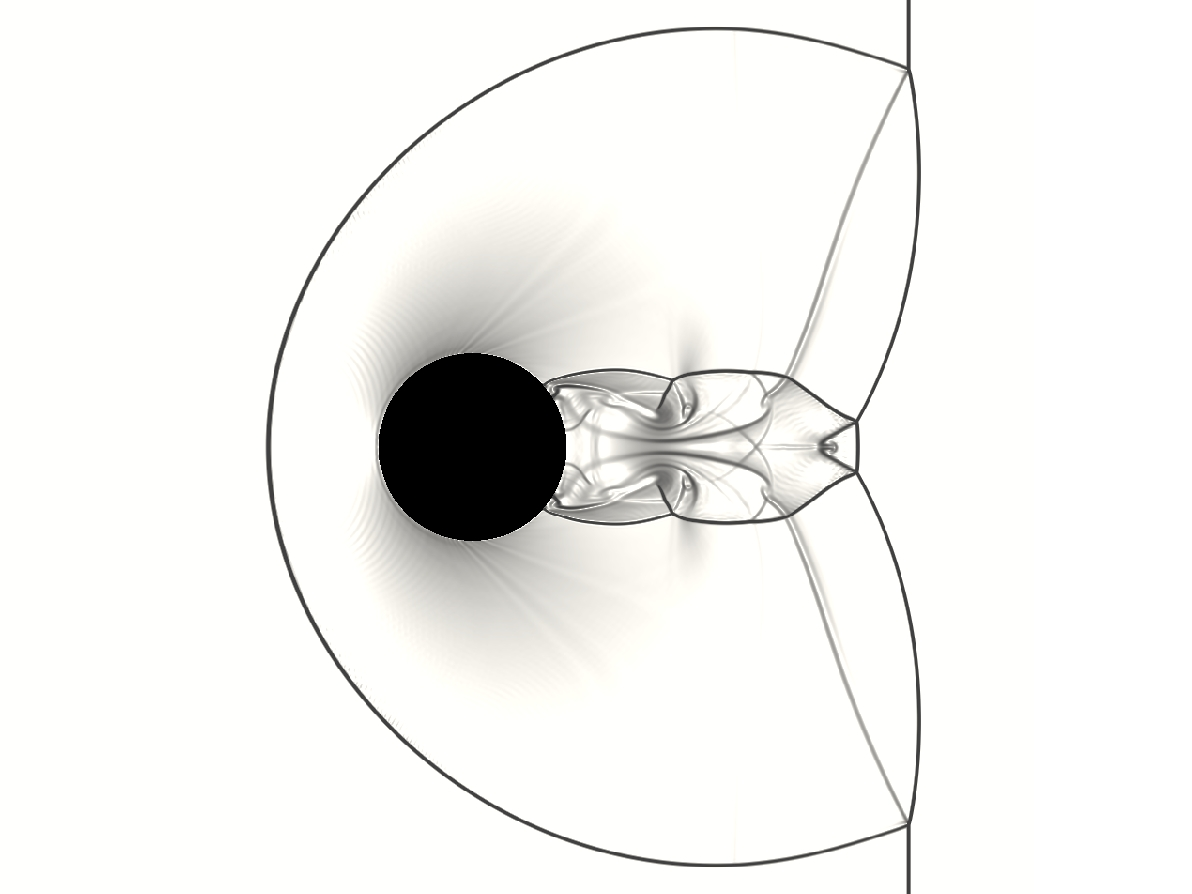
\includegraphics[width=0.40\textwidth]{shock_cyn}
    \bicaption{激波圆柱作用。}{Shock-cylinder interaction.}
    \label{fig:shock_cyn}
\end{figure}

多图的插入如图\ref{fig:oaspl},多图不应在子图中给文本子标题,只要给序号,并在主标题中进行引用说明。
\begin{figure}[!htbp]
    \centering
    \begin{subfigure}[b]{0.35\textwidth}
      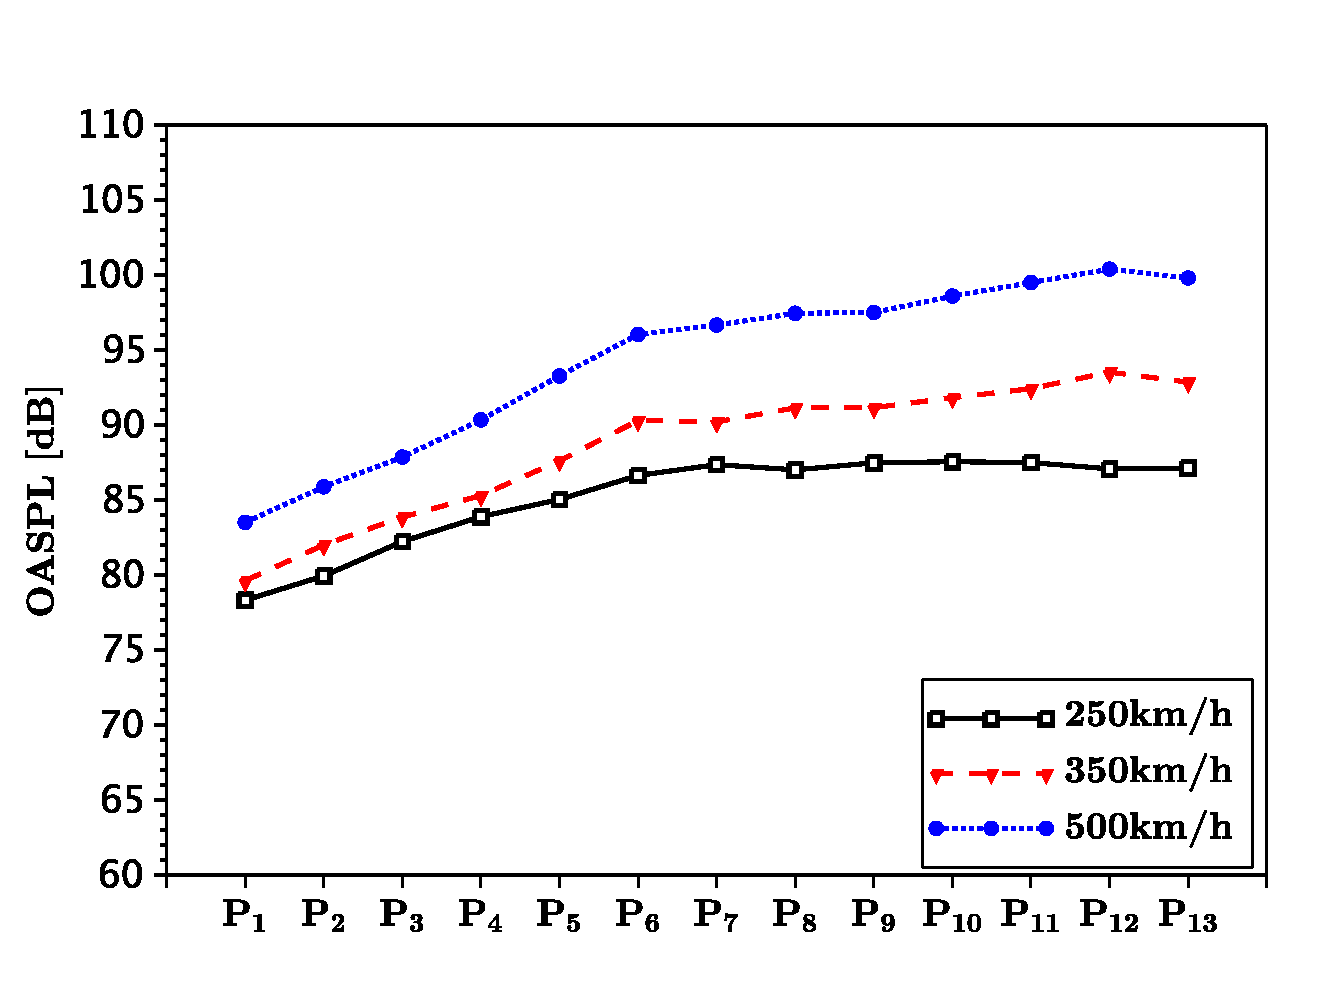
\includegraphics[width=\textwidth]{oaspl_a}
      \caption{}
      \label{fig:oaspl_a}
    \end{subfigure}%
    ~%add desired spacing
    \begin{subfigure}[b]{0.35\textwidth}
      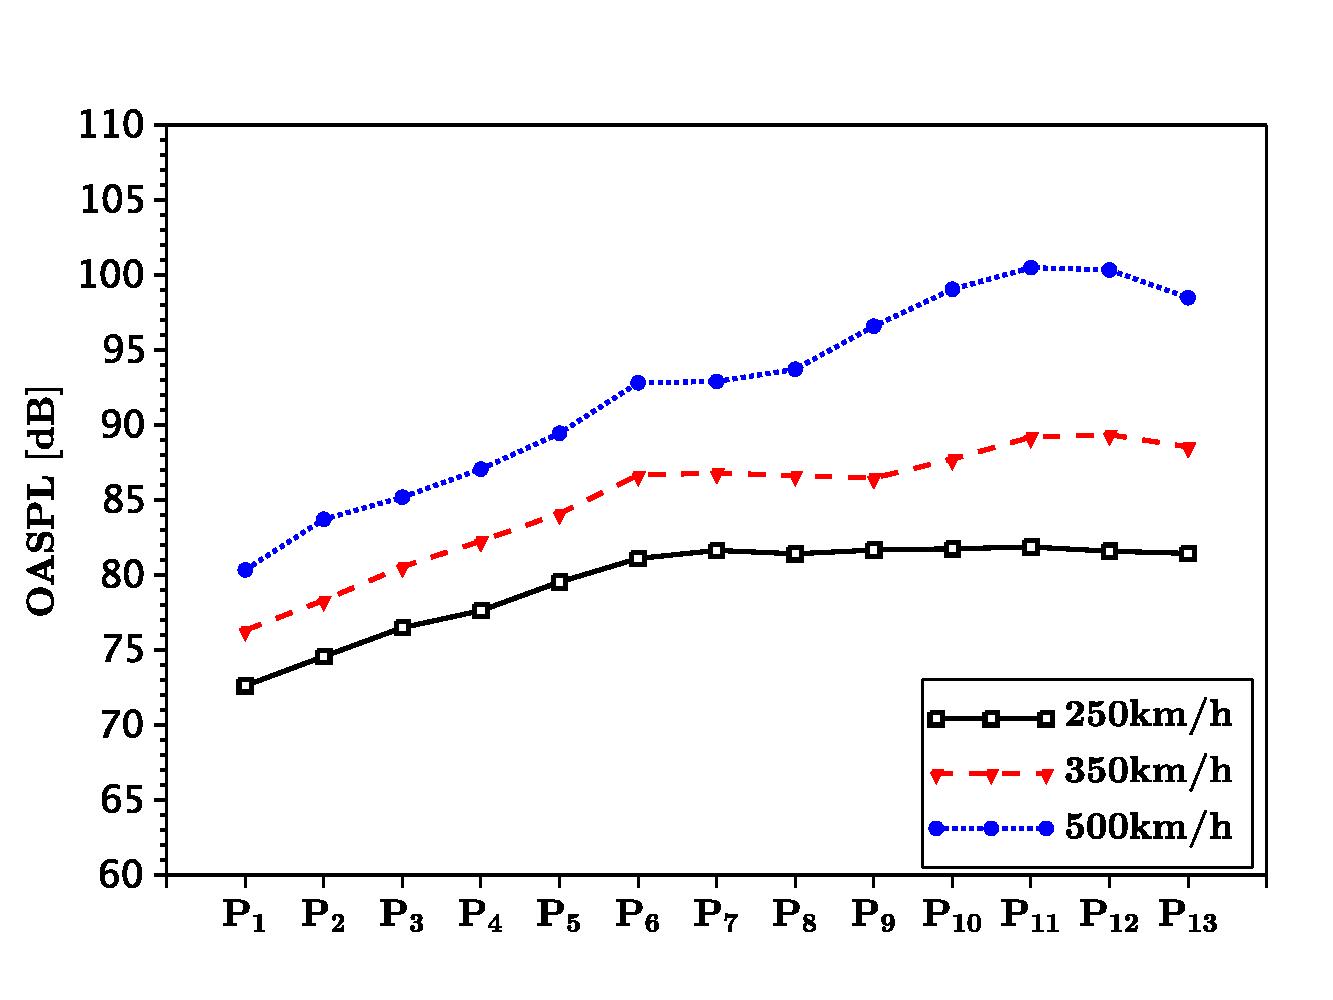
\includegraphics[width=\textwidth]{oaspl_b}
      \caption{}
      \label{fig:oaspl_b}
    \end{subfigure}
    \begin{subfigure}[b]{0.35\textwidth}
      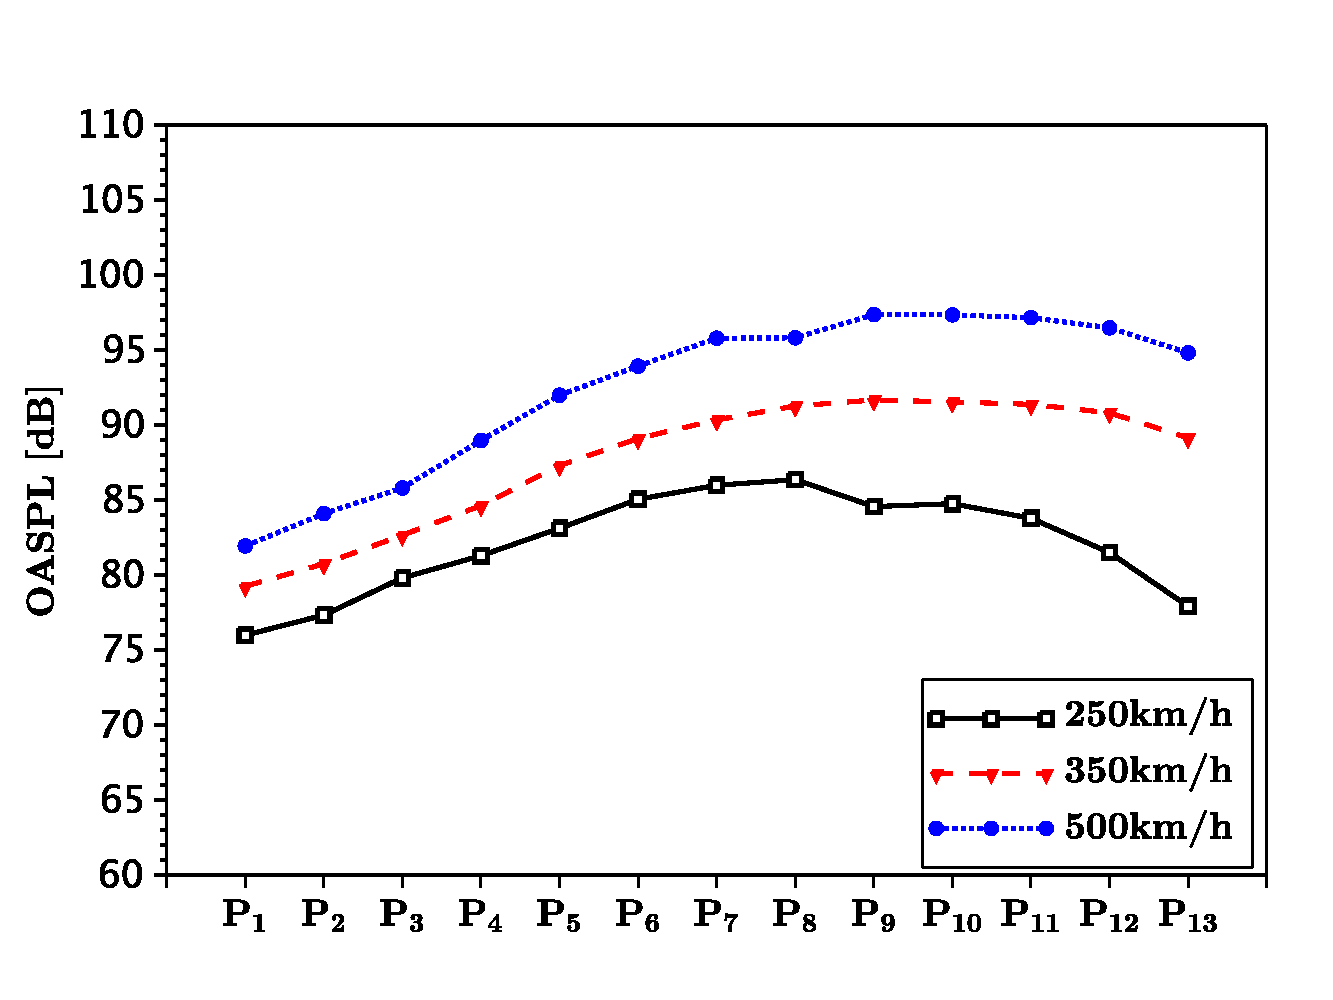
\includegraphics[width=\textwidth]{oaspl_c}
      \caption{}
      \label{fig:oaspl_c}
    \end{subfigure}%
    ~%add desired spacing
    \begin{subfigure}[b]{0.35\textwidth}
      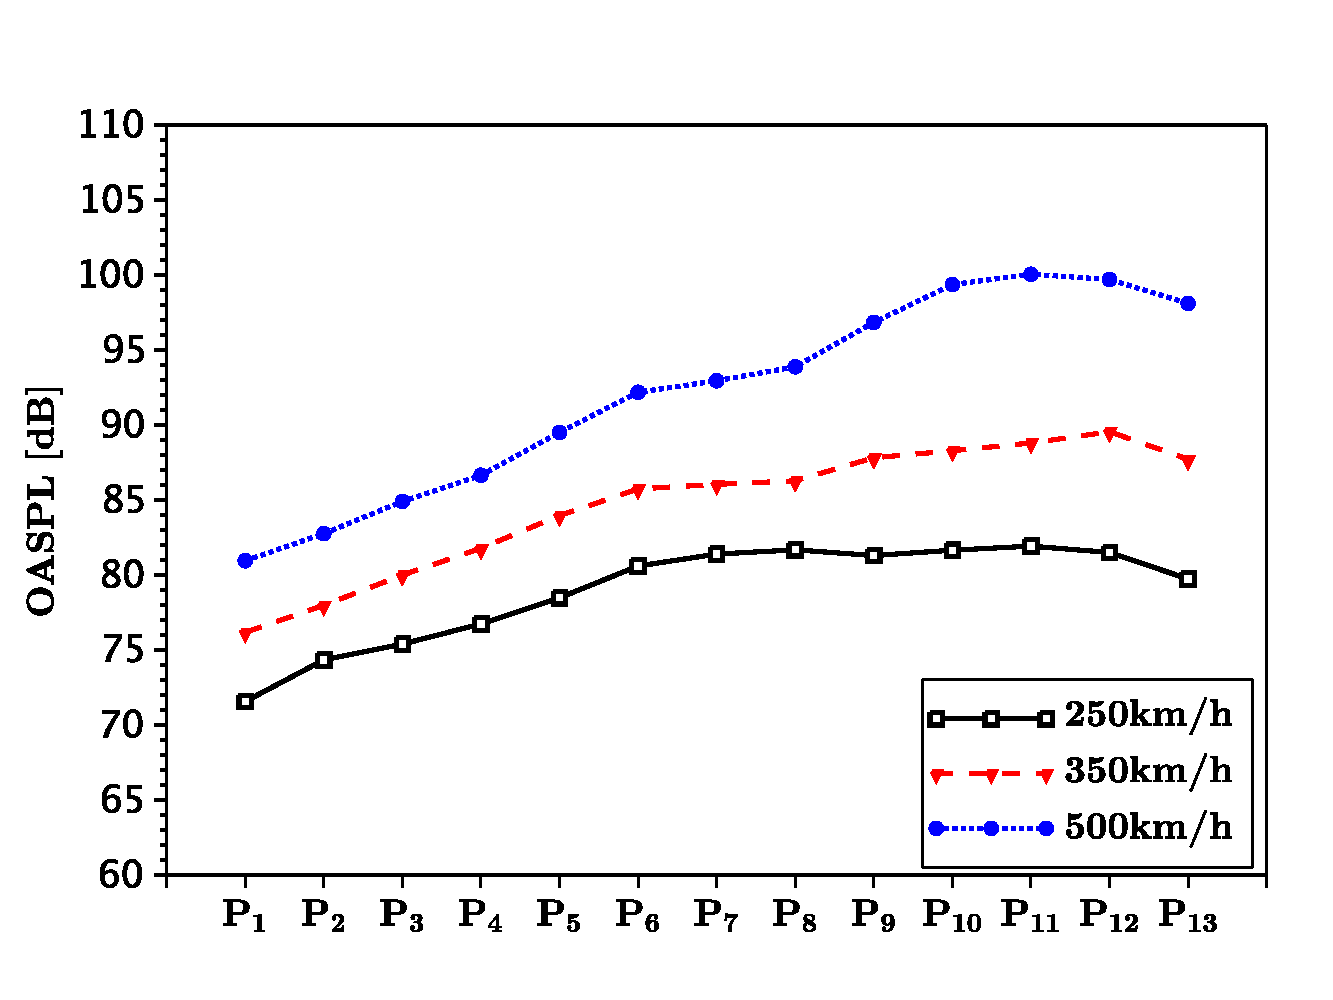
\includegraphics[width=\textwidth]{oaspl_d}
      \caption{}
      \label{fig:oaspl_d}
    \end{subfigure}
    \bicaption{总声压级。(a) 这是子图说明信息,(b) 这是子图说明信息,(c) 这是子图说明信息,(d) 这是子图说明信息。}{OASPL.(a) This is the explanation of subfig, (b) This is the explanation of subfig, (c) This is the explanation of subfig, (d) This is the explanation of subfig.}
    \label{fig:oaspl}
\end{figure}

\subsubsection{表}
表的一般格式是数据依序竖排,内容和项目由左至右横读,通版排版。表号也用章序号编码,如:表2.1是第2章中的第1表。表应有表题,与表号之间空1~2字,置于表的上方居中,用5号宋体,须全文统一。表中的内容和项目字号不大于图题的字号。

请见表~\ref{tab:sample}。制表的更多范例,请见 \href{https://en.wikibooks.org/wiki/LaTeX/Tables}{WiKibook Tables}。
\begin{table}[!htbp]
    \bicaption{这是一个样表。}{This is a sample table.}
    \label{tab:sample}
    \centering
    \footnotesize% fontsize
    \setlength{\tabcolsep}{4pt}% column separation
    \renewcommand{\arraystretch}{1.2}%row space 
    \begin{tabular}{lcccccccc}
        \hline
        Row number & \multicolumn{8}{c}{This is a multicolumn} \\
        %\cline{2-9}% partial hline from column i to column j
        \hline
        Row 1 & $1$ & $2$ & $4$ & $5$ & $6$ & $7$ & $8$\\
        Row 2 & $1$ & $2$ & $4$ & $5$ & $6$ & $7$ & $8$\\
        Row 3 & $1$ & $2$ & $4$ & $5$ & $6$ & $7$ & $8$\\
        Row 4 & $1$ & $2$ & $4$ & $5$ & $6$ & $7$ & $8$\\
        \hline
    \end{tabular}
\end{table}


\subsubsection{公式}
公式包括数学、物理和化学公式。正文中引用的公式、算式或方程式等可以按章序号用阿拉伯数字编号(式号),如:式(2.1)表示第2章第1式,公式一般单行居中排版与上下文分开,式号与公式同行居右排版。

比如Navier-Stokes方程:
\begin{equation} \label{eq:ns}
    \begin{cases}
        \frac{\partial \rho}{\partial t} + \nabla\cdot(\rho\Vector{V}) = 0 \ \mathrm{times\ font\ test}\\
        \frac{\partial (\rho\Vector{V})}{\partial t} + \nabla\cdot(\rho\Vector{V}\Vector{V}) = \nabla\cdot\Tensor{\sigma} \ \text{times font test}\\
        \frac{\partial (\rho E)}{\partial t} + \nabla\cdot(\rho E\Vector{V}) = \nabla\cdot(k\nabla T) + \nabla\cdot(\Tensor{\sigma}\cdot\Vector{V})
    \end{cases}
\end{equation}
\begin{equation}
    \frac{\partial }{\partial t}\int\limits_{\Omega} u \, \mathrm{d}\Omega + \int\limits_{S} \unitVector{n}\cdot(u\Vector{V}) \, \mathrm{d}S = \dot{\phi}
\end{equation}

数学公式常用命令请见 \href{https://en.wikibooks.org/wiki/LaTeX/Mathematics}{WiKibook Mathematics}。artracom.sty中对一些常用数据类型如矢量矩阵等进行了封装,这样的好处是如有一天需要修改矢量的显示形式,只需单独修改artracom.sty中的矢量定义即可实现全文档的修改。

\subsubsection{算法}

如见算法~\ref{alg:euclid},详细使用方法请参见文档 \href{https://ctan.org/pkg/algorithmicx?lang=en}{algorithmicx}。

\begin{algorithm}[!htbp]
    \small
    \caption{Euclid's algorithm}\label{alg:euclid}
    \begin{algorithmic}[1]
        \Procedure{Euclid}{$a,b$}\Comment{The g.c.d. of a and b}
        \State $r\gets a\bmod b$
        \While{$r\not=0$}\Comment{We have the answer if r is 0}
        \State $a\gets b$
        \State $b\gets r$
        \State $r\gets a\bmod b$
        \EndWhile\label{euclidendwhile}
        \State \textbf{return} $b$\Comment{The gcd is b}
        \EndProcedure
    \end{algorithmic}
\end{algorithm}

\subsection{附录}
附录中的图、表、公式、参考文献等另行编排序号,与正文分开,也一律用阿拉伯数字编号,但在数码前冠以附录序码。例如:图A.1,式(B.3)等。
\subsection{计量单位}
学位论文一律采用1984年2月27日国务院发布的《中华人民共和国法定计量单位》,并遵照《中华人民共和国法定计量单位使用方法》执行。论文中命名用各种量、单位和符号,必须遵循国家标准GB3100-82,GB3101-82,GB3102/1-13-82等的规定。

单位名称和符号的书写方式,可以采用国际通用符号,也可以用中文名称,但统一采用一种,不要混用。

\subsection{参考文献}

参考文献引用过程以实例进行介绍,假设需要引用名为"Document Preparation System"的文献,步骤如下:

1)使用Google Scholar搜索Document Preparation System,在目标条目下点击Cite,展开后选择Import into BibTeX打开此文章的BibTeX索引信息,将它们copy添加到ref.bib文件中(此文件位于Biblio文件夹下)。

2)索引第一行 \verb|@article{lamport1986document,|中 \verb|lamport1986document| 即为此文献的label (\textbf{中文文献也必须使用英文label},一般遵照:姓氏拼音+年份+标题第一字拼音的格式),想要在论文中索引此文献,有两种索引类型:

文本类型:\verb|\citet{lamport1986document}|。正如此处所示 \citet{lamport1986document}; 

括号类型:\verb|\citep{lamport1986document}|。正如此处所示 \citep{lamport1986document}。

\textbf{多文献索引用英文逗号隔开}:

\verb|\citep{lamport1986document, chu2004tushu, chen2005zhulu}|。正如此处所示 \citep{lamport1986document,chu2004tushu,chen2005zhulu}

更多例子如:

\citet{walls2013drought}根据...的研究,首次提出...。其中关于...\citep{walls2013drought},是当前中国...得到迅速发展的研究领域\citep{chen1980zhongguo}。引用同一著者在同一年份出版的多篇文献时,在出版年份之后用
英文小写字母区别,如:\citep{yuan2012lana,yuan2012lanb,yuan2012lanc}。同一处引用多篇文献时,按出版年份由近及远依次标注,中间用
分号分开。例如\citep{chen1980zhongguo,stamerjohanns2009mathml,hls2012jinji,niu2013zonghe}。

使用著者-出版年制(authoryear)式参考文献样式时,中文文献必须在BibTeX索引信息的 \textbf{key} 域(请参考ref.bib文件)填写作者姓名的拼音,才能使得文献列表按照拼音排序。参考文献表中的条目(不排序号),先按语种分类排列,语种顺 序是:中文、日文、英文、俄文、其他文种。然后,中文按汉语拼音字母顺序排列,日文按第一著者的姓氏笔画排序,西文和 俄文按第一著者姓氏首字母顺序排列。如中\cite{niu2013zonghe}、日\cite{Bohan1928}、英\cite{stamerjohanns2009mathml}、俄\cite{Dubrovin1906}。

如此,即完成了文献的索引,请查看下本文档的参考文献一章,看看是不是就是这么简单呢?是的,就是这么简单!

不同文献样式和引用样式,如著者-出版年制(authoryear)、顺序编码制(numbers)、上标顺序编码制(super)可在Thesis.tex中对artratex.sty调用实现,如:
\begin{itemize}
    \footnotesize
    \item \verb+\usepackage[numbers]{artratex}+ $\%$ 文本: Jones [1]; 括号: [1]
    \item \verb+\usepackage[super]{artratex}+ $\%$ 文本: Jones 上标[1]; 括号: 上标[1]
    \item \verb+\usepackage[authoryear]{artratex}+ $\%$ 文本: Jones (1995); 括号: (Jones, 1995)
    \item \verb+\usepackage[alpha]{artratex}+ $\%$ 文本: 不可用; 括号: [Jon95]
\end{itemize}

当前文档的默认参考文献样式为\textbf{authoryear}。若在上标(\textbf{super})模式下,希望在特定位置将上标改为嵌入式标,可使用

文本类型:\verb|\citens{lamport1986document,chen2005zhulu}|。

正如此处所示\cite{lamport1986document,chen2005zhulu}

括号类型:\verb|\citens{lamport1986document,chen2005zhulu}|。

正如此处所示\cite{lamport1986document,chen2005zhulu}

参考文献索引更为详细的信息,请见 \href{https://github.com/zepinglee/gbt7714-bibtex-style}{zepinglee} 和 \href{https://en.wikibooks.org/wiki/LaTeX/Bibliography_Management}{WiKibook Bibliography}。


参考文献采用顺序号编号体系。

专著格式: 

[序号] 编著者. 书名[M]. 出版地:出版社,年代,起止页码.

期刊论文格式: 

[序号] 作者. 论文名称[J]. 期刊名称,年度,卷(期):起止页码.

学位论文格式: 

[序号] 作者. 学位论文名称[D]. 发表地:学位授予单位,年度.

参考文献举例: 

[1] 张毅. 铸造工艺CAD及其应用[M]. 北京:机械工业出版社,1994,14-15. 

[2] Huang S C, Huang Y M, Shieh S M. Vibration and stability of a rotating shaft containing a transerse crack [J]. J Sound and Vibration, 1993, 162(3): 387-401.

[3] 周丽. 机械式挖掘机工作装置的优化与仿真[D]. 沈阳:东北大学,2000.


\subsection{攻读博士学位期间取得的学术成果}

期刊格式:
[序号] 作者. 论文名称[J]. 期刊名称,年度,卷(期):起止页码. (检索情况)(对应论文章
节)

专利格式:

[序号] 专利申请者. 专利题名:专利国别,专利号[P]. 发布日期. (对应论文章节)

示例:

[1] Huang S C, Huang Y M, Shieh S M. Vibration and stability of a rotating shaft containing a transerse crack[J]. J Sound and Vibration, 1993, 162(3): 387-401. (SCI检索)(对应论文第四章)

[2] 高航,张立成,周士昌. 高压辊磨机液压系统及其动态特性[J]. 东北大学学报,2000,21(1):38-40. (EI检索)(对应论文第五章)

[3] 刘加林. 多功能一次性压舌板:中国,92214985.2[P]. 1993-04-14. (对应论文第四章)


注:双盲评审版学位论文中须隐去所有作者(申请者)姓名,仅标注排序即可。

示例:

[1] 第一作者. Vibration and stability of a rotating shaft containing a transerse crack[J]. J Sound and Vibration, 1993, 162(3): 387-401. (SCI检索)(对应论文第四章)

[2] 第二作者. 高压辊磨机液压系统及其动态特性[J]. 东北大学学报,2000,21(1):38-40. (EI检索)(对应论文第五章)

[3] 第二排序. 多功能一次性压舌板:中国,92214985.2[P]. 1993-04-14. (对应论文第四章)



